\documentclass[reqno]{amsart}

\usepackage{amsfonts,latexsym,amsthm,amssymb,amsmath,amscd,euscript,bm}
\usepackage[sc]{mathpazo}
\usepackage[margin = 2cm]{geometry}
\usepackage{enumitem}
\usepackage{hyperref}
% sets numbering of enumerate to a, b, c, ...
\renewcommand{\theenumi}{\alph{enumi}}

% Theorems, propositions, etc.
\newtheorem{theorem}{Theorem}
\newtheorem{proposition}[theorem]{Proposition}
\newtheorem{lemma}[theorem]{Lemma}
\newtheorem{corollary}[theorem]{Corollary}

\theoremstyle{definition}
\newtheorem{definition}[theorem]{Definition}
\newtheorem*{claim}{Claim}

\theoremstyle{remark}
\newtheorem*{remark}{Remark}
\newtheorem*{notation}{Notation}

\usepackage{tikz-cd}

\usepackage{thmtools}
\usepackage[framemethod=TikZ]{mdframed}
	\mdfdefinestyle{mdrecbox}
		{%
			linewidth=0.5pt,
			skipabove=12pt,
			frametitleaboveskip=5pt,
			frametitlebelowskip=0pt,
			skipbelow=2pt,
			frametitlefont=\bfseries,
			innertopmargin=4pt,
			innerbottommargin=8pt,
			nobreak=true,
		}
	\declaretheoremstyle
		[
			headfont=\bfseries,
			mdframed={style=mdrecbox},
			headpunct={\\[3pt]},
			postheadspace={0pt},
		]
		{thmrecbox}
\newcounter{problem}[section]	\declaretheorem[style=thmrecbox,name=Problem, numberlike=problem]{statement}


% Solution environment
\newenvironment{solution}
	{
		\begin{proof}[Solution]}{\end{proof}
	}


% Math blackboard font
\newcommand{\nc}{\newcommand}
\nc{\on}[1]{\operatorname{#1}}

\nc{\R}{\mathbb R}
\nc{\C}{\mathbb C}
\nc{\Q}{\mathbb Q}
\nc{\Z}{\mathbb Z}
\nc{\N}{\mathbb N}
\nc{\HH}{\mathbb H}
\nc{\DD}{\mathbb D}
\nc{\TT}{\mathbb T}
\nc{\EE}{\mathbb E}
\nc{\PP}{\mathbb P}

\nc{\cT}{\mathcal T}
\nc{\cA}{\mathcal A}
\nc{\cM}{\mathcal M}
\nc{\cR}{\mathcal R}
\nc{\cB}{\mathcal B}
\nc{\cG}{\mathcal G}
\nc{\cD}{\mathcal D}
\nc{\cS}{\mathcal S}
\nc{\cF}{\mathcal F}
\nc{\cL}{\mathcal L}
\nc{\cE}{\mathcal E}

\nc{\diam}{\operatorname{diam}}
\nc{\del}{\partial}
\nc{\osc}{\operatorname{osc}}
\nc{\inter}{\mathrm{o}}
\nc{\close}[1]{\overline{#1}}
\nc{\supp}{\operatorname{supp}}
\nc{\BV}{\operatorname{BV}}
\nc{\Per}{\operatorname{Per}}
\nc{\loc}{\text{loc}}
\nc{\Lip}{\operatorname{Lip}}
\nc{\ACL}{\operatorname{ACL}}

% Why the f*** would you ever use \epsilon
\renewcommand{\epsilon}{\varepsilon}
\renewcommand{\emph}{\textsc}
\renewcommand{\Re}{\operatorname{Re}}
\renewcommand{\Im}{\operatorname{Im}}
%inverse Fourier transform widecheck
\DeclareFontFamily{U}{mathx}{\hyphenchar\font45}
\DeclareFontShape{U}{mathx}{m}{n}{
      <5> <6> <7> <8> <9> <10>
      <10.95> <12> <14.4> <17.28> <20.74> <24.88>
      mathx10
      }{}
\DeclareSymbolFont{mathx}{U}{mathx}{m}{n}
\DeclareFontSubstitution{U}{mathx}{m}{n}
\DeclareMathAccent{\widecheck}{0}{mathx}{"71}

\let\vec\mathbf

% Title: change problem set number as needed
\title
{
	\emph{Vector fields}
} 

\author{Jason Zhao}
\date{\today}

\begin{document}
\maketitle
\tableofcontents

\section{Vector fields}

Given a smooth manifold $M$, a \emph{vector field} is a smooth assignment of a tangent vector $X_p \in T_p M$ to every point $p \in M$, i.e. $X$ is a section of the tangent bundle. We denote the space of vector fields $\mathfrak X (M)$. In local coordinates $x = (x^1, \dots, x^n)$ on $U \subseteq M$, vector fields take the form
	\[ X_p = X^i (p) \frac{\partial}{\partial x^i} \Big|_{p} \]
where $X^i : U \to \R$ are smooth \emph{component functions} of $X$ in the given coordinates. 

\subsection{Frames}




\subsection{Integral curves}

An \emph{integral curve} $\gamma : I \to M$ of a vector field $X \in \mathfrak X (M)$ is a smooth curve which flows along the field, i.e.
	\[ \frac{d\gamma}{dt} (t) = X_{\gamma(t)}. \]
\begin{center}
\begin{figure}[h]
	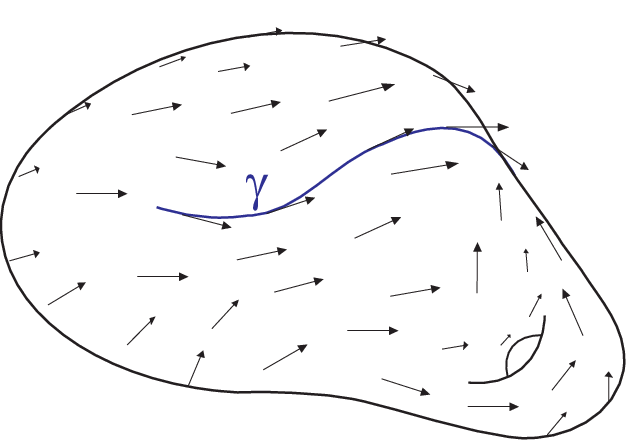
\includegraphics[scale = 0.3]{curve}
	\caption{An integral curve $\gamma$ of a vector field $X$. The \textit{velocity} of the curve at a point $\gamma(t)$ is given exactly by the tangent vector $X_{\gamma(t)}$.}
\end{figure}
\end{center}

\begin{theorem}[Fundamental theorem of ODE]
	Let $X \in \mathfrak X (M)$ be a vector field and $p \in M$, then there exists an open neighborhood $U \subseteq M$ of $p$ and a smooth map $\Phi : U \times (-\epsilon, \epsilon) \to M$ such that, setting
		\[ \gamma_x (t) = \phi_t (x) = \Phi(x, t), \]
	the curves $\gamma_x$ are the unique integral curves of $X$ with initial data $\gamma(0) = x$, and the flows $\phi_t$ are a $1$-parameter group of diffeomorphisms, i.e. $\phi_t \circ \phi_s = \phi_{t + s}$ and $\phi_t^{-1} = \phi_{-t}$. 
\end{theorem}

\begin{remark}
	If $M$ is compact without boundary, then there exists a unique global flow $\Phi : M \times \R \to M$, which we construct by constructing local flows on a finite sub-cover and piecing together by uniqueness to obtain a flow map $\Phi : M \times (-\epsilon, \epsilon) \to M$. Iterating furnishes a flow for all time. 
	
	A counter-example to the existence of a global flow in the non-compact case is $M = \R \setminus 0$ and $X = \tfrac{\partial}{\partial x}$. Viewed on $\R$, the flow $\Phi : \R \times \R \to \R$ is given by 
		\[ \Phi(x, t) = x + t, \]
	which does not restrict to a global flow $\R \setminus 0$ for any time interval $(-\epsilon, \epsilon)$. 	
\end{remark}

\begin{corollary}
	Let $X \in \mathfrak X(M)$ be a vector field and suppose $X(p) \neq 0$ at some point $p \in M$. Then there exist local coordinates in a neighborhood of $p$ such that $X$ is a constant vector field.
\end{corollary}
	
\begin{proof}
	Working in local coordinates $x: U \to \R^n$, suppose that the coordinate function satisfies $X^j (p) \neq 0$. Let $\Sigma \subseteq U$ be the hypersurface given by $x^j = 0$, then restricting the flow $\Phi : (-\epsilon, \epsilon) \times \Sigma \to M$ furnishes a local diffeomorphism. By the inverse function theorem, we obtain coordinates such that 
		\[ X = \frac{\partial}{\partial y^j}. \]	
\end{proof}

\section{Lie algebra}



\subsection{Lie bracket}

Viewing vector fields $X, Y \in \mathfrak X (M)$ as first-order differential operators, i.e. derivations, the \emph{commutator}  of $X$ and $Y$, 
	\[ [X, Y] := XY - YX \]
measures the degree to which $X$ and $Y$ fail to commute. The commutator forms another first-order differential operator $[X, Y] \in \mathfrak X (M)$, which in local coordinates $x$ takes the form
		\[ [X, Y] = \left( X^i \frac{\partial Y^j}{\partial x^i} - Y^i \frac{\partial X^j}{\partial x^i}\right) \frac{\partial}{\partial x^j} .\]
In view of the following properties, 
\begin{itemize}
	\item anti-commutativity, $[X, Y] = - [Y, X]$,
	\item bi-linearity, $[a X + bY, Z] = a[X, Z] + b [Y, Z]$,
	\item the Jacobi identity, $[X, [Y, Z]] + [Y, [Z, X]] + [Z, [X, Y]] = 0$,
\end{itemize}
furnishes a \emph{Lie algebra} structure to the space of vector fields, in which case the commutator is referred to as the \emph{Lie bracket}. One can view the Jacobi identity as describing precisely how associativity fails. 

\begin{proposition}
	
\end{proposition}

\section{Lie derivative}

The \emph{Lie derivative} is the derivative of a tensor field along the flow $\phi_t : M \to M$ of a vector field $X \in \mathfrak X (M)$. The flows define local diffeomorphisms, so the pullback $(\phi_t)^*$ lifts to covariant tensor algebra homomorphism 
	\begin{center}
		\begin{tikzcd}
T^*_{\phi_t (p)}M \arrow[d, hook] \arrow[r, "(\phi_t)^*"] & T^*_{p}M \arrow[d, hook] \\
T(T^*_{\phi_t (p)}M) \arrow[r, "(\phi_t)^*"]              & T(T^*_{p}M)             
\end{tikzcd}
	\end{center}
while the pushforward $(\phi_{-t})_*$ lifts to a contravariant tensor algebra homomorphism 
	\begin{center}
		\begin{tikzcd}
T_{\phi_{-t} (p)}M \arrow[d, hook] \arrow[r, "(\phi_{-t})_*"] & T_{p}M \arrow[d, hook] \\
T(T_{\phi_{-t} (p)}M) \arrow[r, "(\phi_{-t})_*"]              & T(T_{p}M)             
\end{tikzcd}
	\end{center}
The Lie derivative of a section $A \otimes B \in \bigotimes^k T^*M \otimes \bigotimes^l TM$ is defined as
	\[ \mathcal L_X (A \otimes B) = \frac{d}{dt}\Big|_{t = 0} (\phi_t)^* A \otimes \frac{d}{dt}\Big|_{t = 0} (\phi_{-t})_* B. \]
The Lie derivative agrees with the exterior derivative on scalar functions in that if $f \in C^\infty (M)$ then 
	\[ \mathcal L_X f = \frac{d}{dt} \Big|_{t = 0} f(\phi_t) = df (X) = Xf. \]

\subsection{Differential forms}

The Lie derivative of a differential form $\omega \in \Omega^k (M)$ along a vector field $X \in \mathfrak X (M)$ with flow $\phi_t : M \to M$ is given by 
	\[ \mathcal L_X \omega = \frac{d}{dt} \Big|_{t = 0} \phi^*_t \omega. \]
We have already seen that the Lie derivative agrees with the exterior derivative on $0$-forms. The relationship between the two notions of a derivative extends to general $k$-forms via \textit{Cartan's magic formula}. 	
	
\begin{lemma}
	Let $X \in \mathfrak X (M)$, then the Lie derivative $\mathcal L_X : \Omega^k (M) \to \Omega^k (M)$ commutes with the exterior derivative, i.e.
		\[  \mathcal L_X d\omega = d \mathcal L_X \omega,\]
	and satisfies the product rule, 
		\[ \mathcal L_X (\alpha \wedge \beta) = (\mathcal L_X \alpha) \wedge \beta + \alpha \wedge ( \mathcal L_X \beta). \]	
\end{lemma}

\begin{proof}
	The Lie derivative and exterior derivative commute since pullback and differentiating with respect to time commute with the exterior derivative. We verify the product rule by computation, 
		\[ \mathcal L_X (\alpha \wedge \beta) = \frac{d}{dt} \Big|_{t = 0} \phi^*_t (\alpha \wedge \beta) = \frac{d}{dt} \Big|_{t = 0} (\phi^*_t \alpha \wedge \phi^*_t \beta) = (\mathcal L_X \alpha) \wedge \beta + \alpha \wedge ( \mathcal L_X \beta). \]
\end{proof}

\begin{theorem}[Cartan's magic formula]
	Let $\omega \in \Omega^k (M)$ be a $k$-form and suppose $X \in \mathfrak X (M)$ is a vector field, then 
		\[ \mathcal L_X \omega = \iota_X d \omega + d \iota_X \omega. \]
\end{theorem}
	
\begin{proof}
	The operator $\iota_X d + d \iota_X$ agrees with the Lie derivative $\mathcal L_X$ on smooth functions, commutes with the exterior derivative and satisfies the product rule. We prove the result for $1$-forms and induct on degree. Let $\omega \in \Omega^1 (M)$, which in coordinates takes the form
		\[ \omega = f_i dx^i. \]
	Then applying the three properties, we obtain
		\[ \mathcal L_X \omega = \mathcal L_X (f_i dx^i) = \mathcal L_X f_i dx^i + f_i \mathcal L_X dx^i = (\iota_X d + d \iota_X)f_i dx^i + f_i d \mathcal L_X x^i = (\iota_X d + d \iota_X) \omega. \]
	Suppose $k \geq 2$ and Cartan's formula holds on $\Omega^j (M)$ for $j < k$, then writing $\omega \in \Omega^k (M)$ as $\omega = \alpha \wedge \beta$ for some $\alpha \in \Omega^j (M)$ and $\beta \in \Omega^l (M)$ with $0 < j, l < k$ we have
		\[ \mathcal L_X \omega = (\mathcal L_X \alpha) \wedge \beta + \alpha \wedge (\mathcal L_X \beta) = (\iota_X d + d \iota_X) \omega.  \]
	This completes the proof. 
\end{proof}

\begin{proposition}
	Let $\omega \in \Omega^k (M)$ be a differential $k$-form and suppose $X, X_1, \dots, X_k \in \mathfrak X (M)$ are vector fields, then 
		\[ \mathcal L_X (\omega(X_1, \dots, X_k)) = (\mathcal L_X \omega) (X_1, \dots, X_k) + \sum_{i = 1}^k \omega(X_1, \dots, \mathcal L_X X_i, \dots, X_k). \]
\end{proposition}

\begin{proof}
	By Cartan's formula, 
		\begin{align*}
			(\mathcal L_X \omega)(X_1, \dots, X_k)
				&= (\iota_X d + d \iota_X) \omega(X_1, \dots, X_k)
		\end{align*}
		
\end{proof}

\subsection{Vector fields}

\begin{proposition}
	Let $M$ be a manifold and $X, Y \in \mathfrak X (M)$, then 
		\[ \mathcal L_X Y = [X, Y]. \]
\end{proposition}

\begin{proof}
	We compute 
		\begin{alignat*}{2}
			X(Yf)
				&= \mathcal L_X (Yf) \\
				&= \mathcal L_X (df(Y)) \\
				&= (\mathcal L_X df)(Y) + df (\mathcal L_X Y) 
				&&\qquad \text{Cartan's formula} \\
				&= (d \mathcal L_X f) Y + (\mathcal L_X Y) (f) 
				&&\qquad \text{$\mathcal L_X$ commutes with $d$}\\
				&= d(X(f)) Y + (\mathcal L_X Y) (f) \\
				&= Y(Xf) + (\mathcal L_X Y) (f).
		\end{alignat*}
	Rearranging gives the result. 	
\end{proof}

\begin{proposition}
	Let $\omega \in \Omega^k (M)$ and $X_1, \dots, X_{k + 1} \in \mathfrak X (M)$, then 
		\begin{align*}
			d \omega(X_1, \dots, X_{k + 1})
				&= \sum_{i = 1}^k (-1)^{i + 1} X_i (\omega(X_1, \dots, \widehat{X_i}, \dots, X_{k + 1}))\\
				&\qquad + \sum_{i < j} (-1)^{i + j} \omega([X_i, X_j],X_1, \dots, \widehat{X_i}, \dots, \widehat{X_j}, \dots, X_{k + 1}).
		\end{align*}
\end{proposition}
\end{document}